\chapter{Test suite}
\label{ch:testing}

The tests use the \texttt{MATLAB} unit test framework (\code{matlab.unittest}) and need
only base \texttt{MATLAB}.
\begin{lstlisting}
cd tests
run_tests                       % unit + integration tests (about 2 minutes)
run_tests('unit')               % only tests/unit
run_tests('integration')        % only tests/integration
run_tests('KnownIssues', true)  % also tests tagged KnownIssue (open bugs)
run_tests('Coverage', true)     % Cobertura coverage report of code/subroutines
\end{lstlisting}
From the command line or in continuous integration:
\begin{lstlisting}[style=shell]
matlab -batch "cd tests; run_tests"
\end{lstlisting}
\code{run_tests} writes \code{tests/results/junit.xml} (and \code{coverage.xml})
and throws an error if a test fails. On GitHub Actions it also reports every
failed test as an annotation on the run page. It temporarily switches off the
automatic creation of a parallel pool, so the \code{parfor} loops run serially;
pass \code{'Parallel', true} to allow a pool. Every test class puts
\code{code/subroutines} (with subfolders, as \code{SetupPaths} does) and
\code{tests/helpers} on the path with a \code{PathFixture}, so single classes can
also be run with \code{runtests}. GitHub Actions runs the suite on every push
(\code{.github/workflows/tests.yml}).

\section{Unit tests (\texorpdfstring{\texttt{tests/unit}}{tests/unit})}

\begin{xltabular}{\linewidth}{@{}P{5.0cm}L@{}}
  \toprule
  class & what is checked \\
  \midrule
  \endhead
  \code{QuadratureTest} & Gauss-Legendre and Gauss-Lobatto rules integrate
    polynomials of degree $2n-1$ exactly; interval mapping; symmetry \\
  \code{NodalDistributionTest} & node distributions: ascending, symmetric,
    endpoints; GLL nodes are roots of $P_p'$; GLC nodes are Chebyshev extrema;
    unknown distributions are rejected \\
  \code{ShapeFunctionsTest} & 1D/2D Lagrange functions: Kronecker property,
    partition of unity, reproduction of polynomials and their derivatives,
    anisotropic degrees; bilinear and Serendipity functions \\
  \code{MetricShapeFunctionsTest} & metric functions: Kronecker property;
    completeness in $(x,y)$ on distorted elements; finite-difference
    derivatives; equality with the parametric functions on parallelograms; frame
    invariance (rotation, translation, scaling) and the frame dependence of
    \code{method = 0}; skew coordinates \\
  \code{MetricHybridTest} & hybrid trial space (\code{method = 2}): Kronecker
    property, completeness in $(x,y)$ with gradients, finite-difference
    derivatives, frame invariance, Newton inversion when no local coordinates are
    given, equality with the parametric functions (and the classical $\matr K_e$) on
    straight-edged elements, unsymmetry on curved ones, Lebesgue constant $<7$ at
    $p=12$; element matrices: rigid-body modes, rank $n_\mathrm{dof}-3$, \code{KMe_2D} =
    \code{Ke_2D}/\code{Me_2D}, diagonal nodal-quadrature mass, total mass;
    \code{ReferenceNodes2D}, \code{Global2LocalNewton} \\
  \code{MetricBasisTest} & bases of the metric Vandermonde matrix: derivatives,
    span, closed-form values, Lagrange basis equals the parametric 1D functions;
    metric functions independent of the basis and frame invariant for every basis;
    $\matr V$ is a permutation matrix on affine elements up to $p=16$, metric =
    parametric and $\matr K_e$ symmetric at high $p$; Kronecker property on a
    curved element at $p=12$ \\
  \code{GeometryMappingTest} & Jacobian (constant for affine maps, finite
    differences, $\det(\matr J)>0$), node interpolation, element area, inverse
    mapping \\
  \code{MaterialTest} & Hooke matrices: symmetry, positive definiteness, Lamé
    constants, plane stress/strain reduction against closed forms, transverse
    isotropy and rotations \\
  \code{ElementMatricesTest} & rigid-body modes in the right and left null space,
    rank $n_\mathrm{dof}-3$, symmetry on parallelograms (identical to the classical element),
    unsymmetry on distorted elements, constant-strain energy, rotation
    invariance $\matr K' = \matr T\matr K\matr T^{\T}$; mass: total mass,
    symmetry, diagonal GLL nodal quadrature, lumping and its fallbacks \\
  \code{TopologyTest} & DOF and edge connectivity, boundary edges, number and
    position of the high-order nodes on distorted 4- and 8-node meshes, corner
    node numbering \\
  \code{TimeIntegrationTest} & 20 integrators on a 2-DOF oscillator: free
    vibration, step load, convergence order, multiple right-hand sides,
    velocity and acceleration of the central difference method \\
  \code{ExcitationAndDampingTest} & excitation signals and their derivatives
    (finite differences), Rayleigh damping parameters \\
  \code{DriverTest} & building blocks of the program flow:
    \code{MaterialMatrices} (isotropic against closed forms, orthotropic Voigt
    order, invalid plane state), \code{AlignPolynomialDegrees} (aligned and
    rotated neighbours), example parameters of every signal; the shared helpers
    of the time integrators (time step rules, load at an instant, initial
    acceleration, expansion to all DOFs, triangular storage) \\
  \code{CodeHygieneTest} & every file in \code{code/} has help text, no two files
    have the same name (one would shadow the other on the path), every entry of
    \code{TimeIntegrationMethods} exists \\
  \bottomrule
\end{xltabular}

\section{Integration tests (\texorpdfstring{\texttt{tests/integration}}{tests/integration})}

The patch tests and the comparison of the trial spaces in
\cref{sec:metric-hybrid} use a $3\times2$ mesh on $[0,3]\times[0,2]$
(\cref{fig:test-meshes}). Only the interior nodes are moved, so the boundary is
the same for all meshes; the displacements of the exact solution are prescribed
at all boundary nodes, and no other loads act.

\begin{figure}[htbp]
  \centering
  % 3 x 2 test meshes (tests/helpers/usemTestMesh.m, usemDistortMesh.m); generated
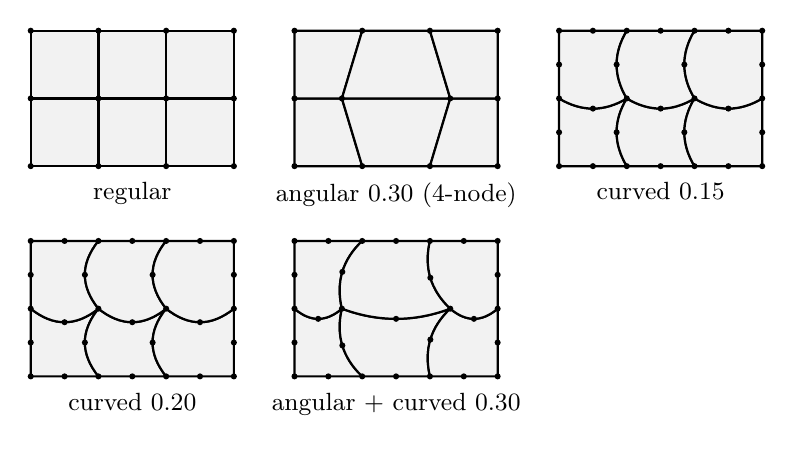
\begin{tikzpicture}[x=0.86cm, y=0.86cm, every node/.style={font=\small}]
  \begin{scope}[xshift=0.00cm, yshift=-0.00cm]
    \draw[thick, fill=black!5] (0.0000,0.0000) -- (1.0000,0.0000) -- (1.0000,1.0000) -- (0.0000,1.0000) -- cycle;
    \draw[thick, fill=black!5] (1.0000,0.0000) -- (2.0000,0.0000) -- (2.0000,1.0000) -- (1.0000,1.0000) -- cycle;
    \draw[thick, fill=black!5] (2.0000,0.0000) -- (3.0000,0.0000) -- (3.0000,1.0000) -- (2.0000,1.0000) -- cycle;
    \draw[thick, fill=black!5] (0.0000,1.0000) -- (1.0000,1.0000) -- (1.0000,2.0000) -- (0.0000,2.0000) -- cycle;
    \draw[thick, fill=black!5] (1.0000,1.0000) -- (2.0000,1.0000) -- (2.0000,2.0000) -- (1.0000,2.0000) -- cycle;
    \draw[thick, fill=black!5] (2.0000,1.0000) -- (3.0000,1.0000) -- (3.0000,2.0000) -- (2.0000,2.0000) -- cycle;
    \fill (0.0000,0.0000) circle (1.1pt);
    \fill (1.0000,0.0000) circle (1.1pt);
    \fill (2.0000,0.0000) circle (1.1pt);
    \fill (3.0000,0.0000) circle (1.1pt);
    \fill (0.0000,1.0000) circle (1.1pt);
    \fill (1.0000,1.0000) circle (1.1pt);
    \fill (2.0000,1.0000) circle (1.1pt);
    \fill (3.0000,1.0000) circle (1.1pt);
    \fill (0.0000,2.0000) circle (1.1pt);
    \fill (1.0000,2.0000) circle (1.1pt);
    \fill (2.0000,2.0000) circle (1.1pt);
    \fill (3.0000,2.0000) circle (1.1pt);
    \node[below] at (1.5,-0.1) {regular};
  \end{scope}
  \begin{scope}[xshift=3.35cm, yshift=-0.00cm]
    \draw[thick, fill=black!5] (0.0000,0.0000) -- (1.0000,0.0000) -- (0.7000,1.0000) -- (0.0000,1.0000) -- cycle;
    \draw[thick, fill=black!5] (1.0000,0.0000) -- (2.0000,0.0000) -- (2.3000,1.0000) -- (0.7000,1.0000) -- cycle;
    \draw[thick, fill=black!5] (2.0000,0.0000) -- (3.0000,0.0000) -- (3.0000,1.0000) -- (2.3000,1.0000) -- cycle;
    \draw[thick, fill=black!5] (0.0000,1.0000) -- (0.7000,1.0000) -- (1.0000,2.0000) -- (0.0000,2.0000) -- cycle;
    \draw[thick, fill=black!5] (0.7000,1.0000) -- (2.3000,1.0000) -- (2.0000,2.0000) -- (1.0000,2.0000) -- cycle;
    \draw[thick, fill=black!5] (2.3000,1.0000) -- (3.0000,1.0000) -- (3.0000,2.0000) -- (2.0000,2.0000) -- cycle;
    \fill (0.0000,0.0000) circle (1.1pt);
    \fill (1.0000,0.0000) circle (1.1pt);
    \fill (2.0000,0.0000) circle (1.1pt);
    \fill (3.0000,0.0000) circle (1.1pt);
    \fill (0.0000,1.0000) circle (1.1pt);
    \fill (0.7000,1.0000) circle (1.1pt);
    \fill (2.3000,1.0000) circle (1.1pt);
    \fill (3.0000,1.0000) circle (1.1pt);
    \fill (0.0000,2.0000) circle (1.1pt);
    \fill (1.0000,2.0000) circle (1.1pt);
    \fill (2.0000,2.0000) circle (1.1pt);
    \fill (3.0000,2.0000) circle (1.1pt);
    \node[below] at (1.5,-0.1) {angular 0.30 (4-node)};
  \end{scope}
  \begin{scope}[xshift=6.71cm, yshift=-0.00cm]
    \draw[thick, fill=black!5] (0.0000,0.0000) .. controls (0.3333,0.0000) and (0.6667,0.0000) .. (1.0000,0.0000) .. controls (0.8000,0.3333) and (0.8000,0.6667) .. (1.0000,1.0000) .. controls (0.6667,0.8000) and (0.3333,0.8000) .. (0.0000,1.0000) .. controls (0.0000,0.6667) and (0.0000,0.3333) .. (0.0000,0.0000) -- cycle;
    \draw[thick, fill=black!5] (1.0000,0.0000) .. controls (1.3333,0.0000) and (1.6667,0.0000) .. (2.0000,0.0000) .. controls (1.8000,0.3333) and (1.8000,0.6667) .. (2.0000,1.0000) .. controls (1.6667,0.8000) and (1.3333,0.8000) .. (1.0000,1.0000) .. controls (0.8000,0.6667) and (0.8000,0.3333) .. (1.0000,0.0000) -- cycle;
    \draw[thick, fill=black!5] (2.0000,0.0000) .. controls (2.3333,0.0000) and (2.6667,0.0000) .. (3.0000,0.0000) .. controls (3.0000,0.3333) and (3.0000,0.6667) .. (3.0000,1.0000) .. controls (2.6667,0.8000) and (2.3333,0.8000) .. (2.0000,1.0000) .. controls (1.8000,0.6667) and (1.8000,0.3333) .. (2.0000,0.0000) -- cycle;
    \draw[thick, fill=black!5] (0.0000,1.0000) .. controls (0.3333,0.8000) and (0.6667,0.8000) .. (1.0000,1.0000) .. controls (0.8000,1.3333) and (0.8000,1.6667) .. (1.0000,2.0000) .. controls (0.6667,2.0000) and (0.3333,2.0000) .. (0.0000,2.0000) .. controls (0.0000,1.6667) and (0.0000,1.3333) .. (0.0000,1.0000) -- cycle;
    \draw[thick, fill=black!5] (1.0000,1.0000) .. controls (1.3333,0.8000) and (1.6667,0.8000) .. (2.0000,1.0000) .. controls (1.8000,1.3333) and (1.8000,1.6667) .. (2.0000,2.0000) .. controls (1.6667,2.0000) and (1.3333,2.0000) .. (1.0000,2.0000) .. controls (0.8000,1.6667) and (0.8000,1.3333) .. (1.0000,1.0000) -- cycle;
    \draw[thick, fill=black!5] (2.0000,1.0000) .. controls (2.3333,0.8000) and (2.6667,0.8000) .. (3.0000,1.0000) .. controls (3.0000,1.3333) and (3.0000,1.6667) .. (3.0000,2.0000) .. controls (2.6667,2.0000) and (2.3333,2.0000) .. (2.0000,2.0000) .. controls (1.8000,1.6667) and (1.8000,1.3333) .. (2.0000,1.0000) -- cycle;
    \fill (0.0000,0.0000) circle (1.1pt);
    \fill (1.0000,0.0000) circle (1.1pt);
    \fill (2.0000,0.0000) circle (1.1pt);
    \fill (3.0000,0.0000) circle (1.1pt);
    \fill (0.0000,1.0000) circle (1.1pt);
    \fill (1.0000,1.0000) circle (1.1pt);
    \fill (2.0000,1.0000) circle (1.1pt);
    \fill (3.0000,1.0000) circle (1.1pt);
    \fill (0.0000,2.0000) circle (1.1pt);
    \fill (1.0000,2.0000) circle (1.1pt);
    \fill (2.0000,2.0000) circle (1.1pt);
    \fill (3.0000,2.0000) circle (1.1pt);
    \fill (0.5000,0.0000) circle (1.1pt);
    \fill (0.8500,0.5000) circle (1.1pt);
    \fill (0.5000,0.8500) circle (1.1pt);
    \fill (0.0000,0.5000) circle (1.1pt);
    \fill (1.5000,0.0000) circle (1.1pt);
    \fill (1.8500,0.5000) circle (1.1pt);
    \fill (1.5000,0.8500) circle (1.1pt);
    \fill (2.5000,0.0000) circle (1.1pt);
    \fill (3.0000,0.5000) circle (1.1pt);
    \fill (2.5000,0.8500) circle (1.1pt);
    \fill (0.8500,1.5000) circle (1.1pt);
    \fill (0.5000,2.0000) circle (1.1pt);
    \fill (0.0000,1.5000) circle (1.1pt);
    \fill (1.8500,1.5000) circle (1.1pt);
    \fill (1.5000,2.0000) circle (1.1pt);
    \fill (3.0000,1.5000) circle (1.1pt);
    \fill (2.5000,2.0000) circle (1.1pt);
    \node[below] at (1.5,-0.1) {curved 0.15};
  \end{scope}
  \begin{scope}[xshift=0.00cm, yshift=-2.67cm]
    \draw[thick, fill=black!5] (0.0000,0.0000) .. controls (0.3333,0.0000) and (0.6667,0.0000) .. (1.0000,0.0000) .. controls (0.7333,0.3333) and (0.7333,0.6667) .. (1.0000,1.0000) .. controls (0.6667,0.7333) and (0.3333,0.7333) .. (0.0000,1.0000) .. controls (0.0000,0.6667) and (0.0000,0.3333) .. (0.0000,0.0000) -- cycle;
    \draw[thick, fill=black!5] (1.0000,0.0000) .. controls (1.3333,0.0000) and (1.6667,0.0000) .. (2.0000,0.0000) .. controls (1.7333,0.3333) and (1.7333,0.6667) .. (2.0000,1.0000) .. controls (1.6667,0.7333) and (1.3333,0.7333) .. (1.0000,1.0000) .. controls (0.7333,0.6667) and (0.7333,0.3333) .. (1.0000,0.0000) -- cycle;
    \draw[thick, fill=black!5] (2.0000,0.0000) .. controls (2.3333,0.0000) and (2.6667,0.0000) .. (3.0000,0.0000) .. controls (3.0000,0.3333) and (3.0000,0.6667) .. (3.0000,1.0000) .. controls (2.6667,0.7333) and (2.3333,0.7333) .. (2.0000,1.0000) .. controls (1.7333,0.6667) and (1.7333,0.3333) .. (2.0000,0.0000) -- cycle;
    \draw[thick, fill=black!5] (0.0000,1.0000) .. controls (0.3333,0.7333) and (0.6667,0.7333) .. (1.0000,1.0000) .. controls (0.7333,1.3333) and (0.7333,1.6667) .. (1.0000,2.0000) .. controls (0.6667,2.0000) and (0.3333,2.0000) .. (0.0000,2.0000) .. controls (0.0000,1.6667) and (0.0000,1.3333) .. (0.0000,1.0000) -- cycle;
    \draw[thick, fill=black!5] (1.0000,1.0000) .. controls (1.3333,0.7333) and (1.6667,0.7333) .. (2.0000,1.0000) .. controls (1.7333,1.3333) and (1.7333,1.6667) .. (2.0000,2.0000) .. controls (1.6667,2.0000) and (1.3333,2.0000) .. (1.0000,2.0000) .. controls (0.7333,1.6667) and (0.7333,1.3333) .. (1.0000,1.0000) -- cycle;
    \draw[thick, fill=black!5] (2.0000,1.0000) .. controls (2.3333,0.7333) and (2.6667,0.7333) .. (3.0000,1.0000) .. controls (3.0000,1.3333) and (3.0000,1.6667) .. (3.0000,2.0000) .. controls (2.6667,2.0000) and (2.3333,2.0000) .. (2.0000,2.0000) .. controls (1.7333,1.6667) and (1.7333,1.3333) .. (2.0000,1.0000) -- cycle;
    \fill (0.0000,0.0000) circle (1.1pt);
    \fill (1.0000,0.0000) circle (1.1pt);
    \fill (2.0000,0.0000) circle (1.1pt);
    \fill (3.0000,0.0000) circle (1.1pt);
    \fill (0.0000,1.0000) circle (1.1pt);
    \fill (1.0000,1.0000) circle (1.1pt);
    \fill (2.0000,1.0000) circle (1.1pt);
    \fill (3.0000,1.0000) circle (1.1pt);
    \fill (0.0000,2.0000) circle (1.1pt);
    \fill (1.0000,2.0000) circle (1.1pt);
    \fill (2.0000,2.0000) circle (1.1pt);
    \fill (3.0000,2.0000) circle (1.1pt);
    \fill (0.5000,0.0000) circle (1.1pt);
    \fill (0.8000,0.5000) circle (1.1pt);
    \fill (0.5000,0.8000) circle (1.1pt);
    \fill (0.0000,0.5000) circle (1.1pt);
    \fill (1.5000,0.0000) circle (1.1pt);
    \fill (1.8000,0.5000) circle (1.1pt);
    \fill (1.5000,0.8000) circle (1.1pt);
    \fill (2.5000,0.0000) circle (1.1pt);
    \fill (3.0000,0.5000) circle (1.1pt);
    \fill (2.5000,0.8000) circle (1.1pt);
    \fill (0.8000,1.5000) circle (1.1pt);
    \fill (0.5000,2.0000) circle (1.1pt);
    \fill (0.0000,1.5000) circle (1.1pt);
    \fill (1.8000,1.5000) circle (1.1pt);
    \fill (1.5000,2.0000) circle (1.1pt);
    \fill (3.0000,1.5000) circle (1.1pt);
    \fill (2.5000,2.0000) circle (1.1pt);
    \node[below] at (1.5,-0.1) {curved 0.20};
  \end{scope}
  \begin{scope}[xshift=3.35cm, yshift=-2.67cm]
    \draw[thick, fill=black!5] (0.0000,0.0000) .. controls (0.3333,0.0000) and (0.6667,0.0000) .. (1.0000,0.0000) .. controls (0.7084,0.2759) and (0.6084,0.6092) .. (0.7000,1.0000) .. controls (0.4667,0.8000) and (0.2333,0.8000) .. (0.0000,1.0000) .. controls (0.0000,0.6667) and (0.0000,0.3333) .. (0.0000,0.0000) -- cycle;
    \draw[thick, fill=black!5] (1.0000,0.0000) .. controls (1.3333,0.0000) and (1.6667,0.0000) .. (2.0000,0.0000) .. controls (1.9084,0.3908) and (2.0084,0.7241) .. (2.3000,1.0000) .. controls (1.7667,0.8000) and (1.2333,0.8000) .. (0.7000,1.0000) .. controls (0.6084,0.6092) and (0.7084,0.2759) .. (1.0000,0.0000) -- cycle;
    \draw[thick, fill=black!5] (2.0000,0.0000) .. controls (2.3333,0.0000) and (2.6667,0.0000) .. (3.0000,0.0000) .. controls (3.0000,0.3333) and (3.0000,0.6667) .. (3.0000,1.0000) .. controls (2.7667,0.8000) and (2.5333,0.8000) .. (2.3000,1.0000) .. controls (2.0084,0.7241) and (1.9084,0.3908) .. (2.0000,0.0000) -- cycle;
    \draw[thick, fill=black!5] (0.0000,1.0000) .. controls (0.2333,0.8000) and (0.4667,0.8000) .. (0.7000,1.0000) .. controls (0.6084,1.3908) and (0.7084,1.7241) .. (1.0000,2.0000) .. controls (0.6667,2.0000) and (0.3333,2.0000) .. (0.0000,2.0000) .. controls (0.0000,1.6667) and (0.0000,1.3333) .. (0.0000,1.0000) -- cycle;
    \draw[thick, fill=black!5] (0.7000,1.0000) .. controls (1.2333,0.8000) and (1.7667,0.8000) .. (2.3000,1.0000) .. controls (2.0084,1.2759) and (1.9084,1.6092) .. (2.0000,2.0000) .. controls (1.6667,2.0000) and (1.3333,2.0000) .. (1.0000,2.0000) .. controls (0.7084,1.7241) and (0.6084,1.3908) .. (0.7000,1.0000) -- cycle;
    \draw[thick, fill=black!5] (2.3000,1.0000) .. controls (2.5333,0.8000) and (2.7667,0.8000) .. (3.0000,1.0000) .. controls (3.0000,1.3333) and (3.0000,1.6667) .. (3.0000,2.0000) .. controls (2.6667,2.0000) and (2.3333,2.0000) .. (2.0000,2.0000) .. controls (1.9084,1.6092) and (2.0084,1.2759) .. (2.3000,1.0000) -- cycle;
    \fill (0.0000,0.0000) circle (1.1pt);
    \fill (1.0000,0.0000) circle (1.1pt);
    \fill (2.0000,0.0000) circle (1.1pt);
    \fill (3.0000,0.0000) circle (1.1pt);
    \fill (0.0000,1.0000) circle (1.1pt);
    \fill (0.7000,1.0000) circle (1.1pt);
    \fill (2.3000,1.0000) circle (1.1pt);
    \fill (3.0000,1.0000) circle (1.1pt);
    \fill (0.0000,2.0000) circle (1.1pt);
    \fill (1.0000,2.0000) circle (1.1pt);
    \fill (2.0000,2.0000) circle (1.1pt);
    \fill (3.0000,2.0000) circle (1.1pt);
    \fill (0.5000,0.0000) circle (1.1pt);
    \fill (0.7063,0.4569) circle (1.1pt);
    \fill (0.3500,0.8500) circle (1.1pt);
    \fill (0.0000,0.5000) circle (1.1pt);
    \fill (1.5000,0.0000) circle (1.1pt);
    \fill (2.0063,0.5431) circle (1.1pt);
    \fill (1.5000,0.8500) circle (1.1pt);
    \fill (2.5000,0.0000) circle (1.1pt);
    \fill (3.0000,0.5000) circle (1.1pt);
    \fill (2.6500,0.8500) circle (1.1pt);
    \fill (0.7063,1.5431) circle (1.1pt);
    \fill (0.5000,2.0000) circle (1.1pt);
    \fill (0.0000,1.5000) circle (1.1pt);
    \fill (2.0063,1.4569) circle (1.1pt);
    \fill (1.5000,2.0000) circle (1.1pt);
    \fill (3.0000,1.5000) circle (1.1pt);
    \fill (2.5000,2.0000) circle (1.1pt);
    \node[below] at (1.5,-0.1) {angular + curved 0.30};
  \end{scope}
\end{tikzpicture}

  \caption{$3\times2$ test meshes (\texttt{usemTestMesh}, \texttt{usemDistortMesh}):
    4-node meshes (regular, angular distortion 0.30) and 8-node meshes with
    curved-edge distortion (mid-side nodes moved normal to their edge by 0.15 or
    0.20) and with combined angular and curved-edge distortion. Dots: nodes of
    the input mesh. Boundary condition: prescribed displacements on the whole
    boundary.}
  \label{fig:test-meshes}
\end{figure}

\begin{xltabular}{\linewidth}{@{}P{5.0cm}L@{}}
  \toprule
  class & what is checked \\
  \midrule
  \endhead
  \code{PatchTest} & displacement patch tests on regular, angular, curved and
    combined distorted meshes for $p = 1,\dots,4$, plane stress and plane strain:
    linear fields, all harmonic fields $(\operatorname{Re}(z^k), -\operatorname{Im}
    (z^k))$ with $k\le p$, and pure bending are reproduced to machine precision.
    Control experiment: the classical symmetric element fails on the same curved
    mesh. Fields of higher degree are not exact; exponential $p$-convergence for
    $(e^x\cos(y), -e^x\sin(y))$. All exactness and convergence tests run for both
    trial spaces (\code{method} 1 and 2); the hybrid element equals the classical one
    on the angular mesh and is unsymmetric on the curved mesh \\
  \code{RunSimulationTest} & the complete program flow from the input file:
    static result against the stored reference solution, modal analysis against
    the dense eigenvalues of the returned matrices, frequency-domain solution for
    $\omega\to0$ against the static one, transient analysis (Newmark), saved
    files (results, $u_y$ export, solver input that reproduces the time
    integration), errors for an unknown analysis type and a missing input file \\
  \code{LeeBathePatchTest} & the Lee-Bathe patch tests (reference data in
    \code{tests/fixtures/reference}), repeated with the steps of
    \code{StaticAnalysis}: the quadratic test matches the analytical pure-bending
    solution for all meshes and $p\ge2$; the cubic test for $p = 3$ is
    mesh-independent and matches the stored solution; both trial spaces \\
  \code{AbaqusInputTest} & end to end: the input files in
    \code{code/InputFilesAbaqus} are read with \code{ReadModel}, lifted to degree
    $p$ and compared with the reference models; static analysis from the input
    file \\
  \code{AbaqusReaderTest} & reader robustness with modified input files: exact set
    names (\code{Set-1} vs.\ \code{Set-10}), missing sets (error instead of an
    endless loop), U2 + U3 in separate lines, \texttt{\%} in the file, node labels,
    gravity, \code{*Cload} on a generated set \\
  \code{DirichletBCTest} & homogeneous and prescribed displacements
    (elimination), uniaxial stretch on a distorted mesh, node sets used as given \\
  \code{LoadsTest} & body forces on element subsets, several body forces, gravity
    with the density of each material, one or several load cases, amplitude of
    spatially varying loads \\
  \code{SolverTransientTest} & \code{Solver_Transient} with the input struct of
    \code{DynamicAnalysis} or its MAT file: methods 301, 306, 202, 402, 403
    (undamped and damped Padé, also from rest under a constant load), 109 with
    element data (and the error without), all DOFs saved with
    \code{save_var = 1}, Newmark fallback (with a warning) for unknown codes,
    unique method codes \\
  \code{AdaptiveHybridExplicitTest} & adaptive hybrid explicit method:
    second-order convergence, mass-proportional damping against the exact
    solution, stable and accurate at twice the critical time step of the central
    difference method (which diverges), diagonal lumped mass \\
  \bottomrule
\end{xltabular}

\section{Helpers and fixtures}

\begin{xltabular}{\linewidth}{@{}P{5.0cm}L@{}}
  \toprule
  file & purpose \\
  \midrule
  \code{helpers/usemTestMesh} & structured 4- or 8-node mesh in \texttt{ABAQUS} node order \\
  \code{helpers/usemDistortMesh} & deterministic angular, curved-edge or combined
    distortion of interior nodes \\
  \code{helpers/usemTestElement} & single test elements (square, parallelogram,
    trapezoid, curved, general) \\
  \code{helpers/usemBuildModel} & wrapper of \code{pSpectralElement_NodesTopology} \\
  \code{helpers/usemAssemble} & quiet wrapper of \code{AssemblyFEM} \\
  \code{helpers/usemDirichletSolve} & displacement-driven patch test \\
  \code{helpers/usemKeSymmetric} & classical (Bubnov-Galerkin) element stiffness,
    for comparisons only \\
  \code{helpers/usemReadAbaqus} & \code{ReadModel} without progress output (used
    by the studies) \\
  \code{fixtures/reference/*.mat} & model data and solutions of the Lee-Bathe
    tests, extracted from the result workspaces in
    \code{code/subroutines/Results/Static} (\code{make_reference_fixtures.m}) \\
  \code{fixtures/make_abaqus_inputs.m} & generation of the \texttt{ABAQUS} input files
    from the fixtures \\
  \bottomrule
\end{xltabular}

\section{Writing new tests}

\begin{itemize}
  \item Put the new class in \code{tests/unit} or \code{tests/integration} and copy
    the \code{TestClassSetup} block (path fixtures) from an existing class.
  \item Wrap routines that print progress (\code{AssemblyFEM}, \code{NeumannBCs},
    integrators, \code{RunSimulation}) in \code{evalc}, or use the helpers that
    already do this; for \code{RunSimulation} also set \code{settings.verbose},
    \code{settings.parallel}, \code{settings.saveWS} and the plot flags to
    \code{false}.
  \item Numerical changes that should not change results (refactoring) can be
    checked bit for bit against the unmodified code: run both versions on the
    same input and compare with \code{isequal}, as \code{RunSimulationTest} and
    \code{SolverTransientTest} do for files written by the program.
  \item Use deterministic meshes (\code{usemDistortMesh}) or a seeded
    \code{RandStream}.
  \item Use only base \texttt{MATLAB} functions (the GitHub runner has no toolboxes).
  \item Tag tests that document an unfixed bug with
    \code{TestTags = {'KnownIssue'}} and describe the bug in \cref{ch:issues}.
\end{itemize}
